% Editing notes
% - No tabs, just spaces!
% - No hanging whitespace
% - Wrap lines to 79 characters
% - Indentation should be two spaces per indent
% - Only one space after periods.
% - Don't worry about formatting details, just get the content in place.

% 12pt font is recommend for the preprint
\documentclass[fleqn,12pt]{wlpeerj}

% for the preprint we add line numbers
\usepackage{lineno}
\linenumbers

% for images: png, pdf, etc
\usepackage{graphicx}

% for nice table formatting, i.e. /toprule, /midrule, etc
\usepackage{booktabs}

% to allow for \verb++ declarations in captions.
\usepackage{cprotect}

% for nice source code syntax highlighting, also provides Listing env
\usepackage{minted}

% for nice units
\usepackage{siunitx}

\title{An elaborate data set on human gait and the effect of mechanical
  perturbations}

\author[1]{Jason K. Moore}
\author[1]{Sandra K. Hnat}
\author[1]{Antonie J. van den Bogert}

\affil[1]{Mechanical Engineering, Cleveland State University, Cleveland, Ohio,
  USA, 44115. j.k.moore19@csuohio.edu, s.hnat@vikes.csuohio.edu,
  a.vandenbogert@csuohio.edu}

\keywords{gait, data, perturbation}

\begin{abstract}

  Here we share a rich gait data set collected from fifteen subjects walking at
  three speeds on an instrumented treadmill. Each trial consists of 120 seconds
  of normal walking and 480 seconds of walking while being longitudinally
  perturbed during each stance phase with pseudo-random fluctuations in the
  speed of the treadmill belt. A total of approximately 1.5 hours of normal
  walking ($>5000$ gait cycles) and 6 hours of perturbed walking ($>20,000$
  gait cycles) is included in the data set. We provide full body marker
  trajectories and ground reaction loads in addition to a presentation of
  processed data that includes gait events, 2D joint angles, angular rates, and
  joint torques along with the open source software used for the computations.
  The protocol is described in detail and supported with additional elaborate
  meta data for each trial. This data can likely be useful for validating or
  generating mathematical models that are capable of simulating normal periodic
  gait and non-periodic, perturbed gaits.

\end{abstract}

\begin{document}

\flushbottom
\maketitle
\thispagestyle{empty}

\section*{Introduction}
%
The collection of dynamical data during human walking has a long history
beginning with the first motion pictures and now with modern marker based
motion capture techniques and high fidelity ground reaction load measurements.
Even though years of data on thousands of subjects now exist, this data is not
widely disseminated, well organized, nor available with few or no restrictions.
David Winter's published normative gait data, \cite{Winter1990}, is widely used
in biomechanical studies, yet it comes from relatively few subjects and only a
small number of gait cycles per subject. This small source has successfully
inspired many other studies, such as powered prosthetic control
design, \cite{Sup2008}, but success in other research fields using large sets
of data for discovery lead one to believe that more elaborate data sets may
benefit the field of human motion studies. To enable such work, biomechanical
data needs to be shared extensively, organized, and curated to enable future
analysts.

There are some notable gait data sets and databases besides Winter's
authoritative set that are publicly available. The International Society of
Biomechanics has maintained a web page (http://isbweb.org/data) since
approximately 1995 that includes data sets for download and mostly unencumbered
use. For example, Vaughn, et. al's data, \cite{Vaughan1992}, with kinematics
and force plate measurement from several subjects is available on the site. At
another website, the CGA Normative Gait Database, \cite{Kirtley2014} shares
normative gait data from several studies and these files have influenced other
studies, for example the average gait cycles from children used in
\cite{Bogert2003}.

\cite{Chester2007} report on a large gait database comparison where one
database contained kinematic data of 409 gait cycles of children from 1 to 7
years old but the data does not seem to be publicly available. This is
unfortunately typical. But Tirosh et. al, recognized the need for a
comprehensive data base for clinical gait data and created the Gaitabase,
\cite{Tirosh2010}. This database may contain a substantial amount of data but
it is encumbered by a very complicated and restrictive license and sharing
scheme. However, there are examples of data with less restrictions. The
University of Wisconsin at LaCrosse has an easily accessible normative gait
data set, \cite{Willson2014}, from 25 subjects with lower extremity marker data
from multiple gait cycles and force plate measurements from a single gait
cycle.

More recent examples of biomechanists sharing their data alongside publications
are: \cite{Bogert2013} which includes full body joint kinematics and kinetics
from eleven subjects walking for a small number of gait cycles and
\cite{Wang2014} who includes a larger set of data from ten subjects walking for
five minutes each at three different speeds but only a small set of lower
extremity markers are present. The second is notable because it publishes the
data in Dryad, a modern citable data repository.

The publicly available gait data is small compared to the number of gait
studies that have been performed over the years. The data that is available
generally suffers from limitations such as few subjects, few gait cycles, few
markers, highly clinical, no raw data, limited force plate measurements, lack
of meta data, non-standard formats, and restrictive licensing. To help with
this situation we are making the data we collected for our research purposes
publicly available and free of the previously mentioned deficiencies. Not only
do we provide a larger set of normative gait data that has been previously
available, we also include an even larger set of data in which the subject is
being perturbed, something that does not currently exist. We believe both of
these sets of data can serve a variety of use cases and hope that we can save
time and effort for future researchers by sharing it.

Our use case for the data is centered around the need of bio-inspired control
systems for emerging powered prosthetics and orthotics. Ideally, a powered
prosthetic would behave in such a way that the user would feel like their limb
was never disabled. There are a variety of approaches to developing
bio-inspired control systems, some of which aim to mimic the reactions and
motion of an able-bodied person. A modern gait lab is able to collect a variety
of kinematic, kinetic, and physiological data from humans during gait. This
data can potentially be used to drive the design of the human-mimicking
controller. With a rich enough data set, one may be able to identify control
mechanisms used during a human's natural gait and recovery from perturbations.
We have collected data that is richer than previous gait data sets and may be
rich enough for control identification. The data can also be used for
verification purposes for controllers that have been designed in other manners.

With all of this in mind, we collected over seven and half hours of gait data
from fifteen able bodied subjects which amounts to over 25,000 gait cycles. The
subjects walked at three different speeds on an instrumented treadmill while we
collected full body marker locations and ground reaction loads from a pair of
force plates. The protocol for the majority of the trials included two minutes
of normal walking and eight minutes of walking under the influence of
pseudo-random belt speed fluctuations. The data has been organized complete
with rich meta data and made available in the most unrestrictive form for other
research uses following modern best practices in data sharing, \cite{White2013}.

Furthermore, we include a small Apache licensed open source software library
for basic gait analysis and demonstrate its use in the paper. The combination
of the open data and open software allow the results presented within to be
computationally reproducible and instructions are included in the associated
repository for doing so.

\section*{Methods}
\subsection*{Participants}
%
Fifteen able bodied subjects including four females and eleven males with an
average age of $24\pm4$ years, height of $1.75\pm0.09$ m, mass of $74\pm13$ kg
participated in the study. The study was approved by the Institutional Review
Board of Cleveland State University (\# 29904-VAN-HS) and written informed
consent was obtained from all participants. The data has been anonymized with
respect to the participants' identities and a unique identification number was
assigned to each subject. A selection of the meta data collected for each
subject is shown in Table~\ref{tab:subjects}.
%
\begin{table}
  \cprotect\caption{Information about the 15 participants. The final three
    columns provide the trial numbers associated with each nominal treadmill
    speed. The measured mass is computed from the mean total vertical ground
    reaction force just after the calibration pose event, if possible. If the
    mass is reported without an accompanying standard deviation, it is the
    subject's self-reported mass. Additional trials found in the data set with
    a subject identification number 0 are trials with no subject, i.e.
    unloaded trials that can be used for inertial compensation purposes, and
    are not shown in the table. Generated
    by \verb|src/subject_table.py|.}
  \centering
  \small
  \begin{tabular}{rlrrrrlll}
\toprule
 Id &  Gender &  Age [yr] & Height [m] &            Measured Mass [kg] &  Self-reported mass [kg] & 0.8 m/s &  1.2 m/s & 1.6 m/s \\
\midrule
    &         &           &            &                               &                          &         &          &         \\
  1 &    male &        25 &       1.87 &                            NA &                  101.000 &      NA &  6, 7, 8 &      NA \\
  3 &  female &        32 &       1.62 &      $54\pm2$ &                   60.000 &      46 &       47 &      48 \\
  4 &    male &        30 &       1.76 &                            NA &                   74.000 &  12, 15 &       13 &      14 \\
  5 &    male &        23 &       1.73 &  $71.2\pm0.9$ &                   65.000 &      32 &       31 &      33 \\
  6 &    male &        26 &       1.77 &  $86.8\pm0.6$ &                   80.000 &      40 &       41 &      42 \\
  7 &  female &        29 &       1.72 &  $64.5\pm0.8$ &                   63.000 &      16 &       17 &      18 \\
  8 &    male &        20 &       1.57 &  $74.9\pm0.9$ &                   70.000 &      19 &       20 &      21 \\
  9 &    male &        20 &       1.69 &      $67\pm2$ &                   64.000 &      25 &       26 &      27 \\
 10 &    male &        19 &       1.77 &      $92\pm2$ &                   90.700 &      61 &       62 &      63 \\
 11 &    male &        22 &       1.85 &                            NA &                   80.000 &       9 &       10 &      11 \\
 12 &    male &        22 &       1.85 &  $74.2\pm0.5$ &                   81.000 &      49 &       50 &      51 \\
 13 &  female &        21 &       1.70 &      $58\pm2$ &                   64.000 &      55 &       56 &      57 \\
 15 &    male &        22 &       1.83 &  $80.5\pm0.8$ &                   79.400 &      67 &       68 &      69 \\
 16 &  female &        28 &       1.69 &  $56.2\pm0.6$ &                   52.160 &      76 &       77 &      78 \\
 17 &    male &        23 &       1.86 &  $88.3\pm0.8$ &                   86.999 &      73 &       74 &      75 \\
\bottomrule
\end{tabular}

  \label{tab:subjects}
\end{table}
%
\begin{table}
  \cprotect\caption{A list of unloaded trials collected for each speed. Each
    loaded trial includes a compensation file listed in its meta data which
    matches it to these unloaded trials. Generated by
    \verb|src/subject_table.py|.}
  \centering
  \small
  \begin{tabular}{rr}
\toprule
Speed & Trial Numbers \\
\midrule
0.8 m/s & 22, 30, 34, 43, 52, 58, 64, 70, 79 \\
1.2 m/s & 3, 4, 5, 23, 29, 35, 44, 53, 59, 65, 71, 80 \\
1.6 m/s & 24, 28, 36, 45, 54, 60, 66, 72, 81 \\
\bottomrule
\end{tabular}
  \label{tab:comptrials}
\end{table}

\subsection*{Equipment}
%
The data were collected in the Laboratory for Human Motion and Control at
Cleveland State University, using the following equipment:
%
\begin{itemize}
  \item A R-Mill treadmill which has dual 6 degree of freedom force plates,
    independent belts for each foot, and lateral/pitch motion capabilities
    (Forcelink, Culemborg, Netherlands).
  \item A 10 Osprey camera motion capture system paired with the Cortex
    3.1.1.1290 software (Motion Analysis, Santa Rosa, CA, USA).
  \item USB-6255 data acquisition unit (National Instruments, Austin, Texas,
    USA).
  \item Four ADXL330 Triple Axis Accelerometer Breakout boards attached to the
    treadmill (Sparkfun, Niwot, Colorado, USA).
  \item D-Flow software (versions 3.16.1 to 3.16.2) and visual display system,
    (Motek Medical, Amsterdam, Netherlands).
\end{itemize}

The Cortex software delivers high accuracy 3D marker trajectories from the
cameras along with data from force plates and analog sensors
(EMG/Accelerometer) through a National Instruments USB-6255 data acquisition
unit. D-Flow is required to collect data from any digital sensors and to
control the treadmill's motion (lateral, pitch, and belts). D-Flow can process
the data in real time and/or export data to file.

Our motion capture system's coordinate system is such that the X coordinate
points to the right, the Y coordinate points upwards, and the Z coordinate
follows from the right-hand-rule, i.e. points backwards with respect to the
walking direction. The camera's coordinate system is aligned to an origin point
on treadmill's surface during camera calibration. The same point is used as the
origin of the ground reaction force measuring system.
Figure~\ref{fig:treadmill} shows the layout of the equipment.

Early on, we discovered that the factory setup of the R-Link treadmill had a
vibration mode as low as 5\si{\hertz} that is detectable in the force measurements,
likely due to the flexible undercarriage and pitch motion mechanism. Trials 6-8
are affected by this vibration mode. During trials 9-15 the treadmill was
stabilized with wooden blocks. During the remaining trials the treadmill was
stabilized with metal supports. See the Data Limitations Section for more
details.

The acceleration of the treadmill was measured during each trial by four
ADXL330 accelerometers placed at the four corners of the machine. These
accelerometers were intended to provide information for inertial compensation
purposes when the treadmill moved laterally, but are extraneous for trials
greater than 8 due to the treadmill being stabilized.
%
\begin{figure}
  \centering
  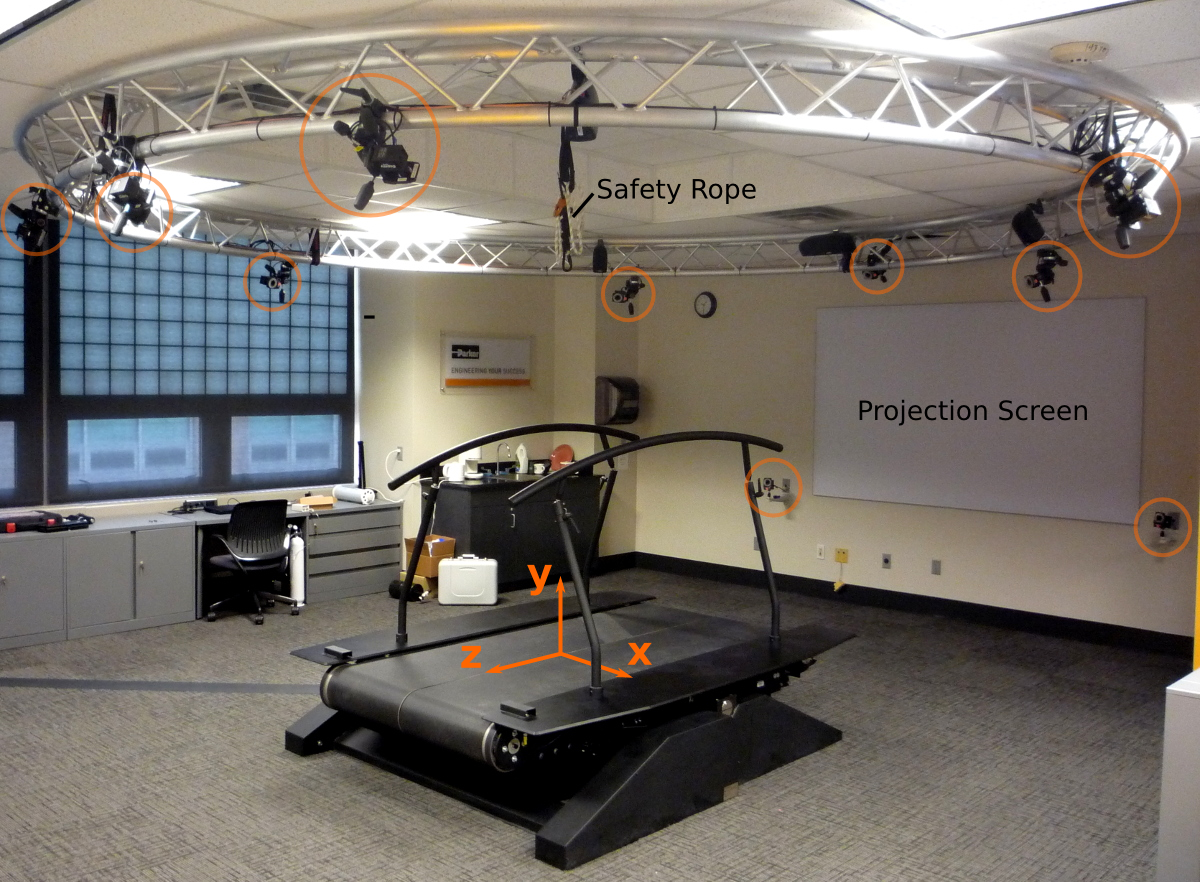
\includegraphics{figures/treadmill.png}
  \caption{The treadmill with coordinate system, cameras (circled in orange),
    projection screen, and safety rope. The direction of travel is in the $-z$
    direction.}
  \label{fig:treadmill}
\end{figure}

\subsection*{Protocol}
%
The experimental protocol consisted of both static measurements and walking on
the treadmill for 10 minutes under unperturbed and perturbed conditions. Before
a set of trials on the same day the following happened:
%
\begin{itemize}
  \item Calibration of the motion capture system using the manufacturer's
    recommended procedure.
  \item Subject changes into athletic shoes, shorts, sports bra, baseball
    cap, and rock climbing harness.
  \item All 47 markers are applied directly to the skin except for the heel,
    toe, and head markers, which were placed on the respective article of
    clothing.~\footnote{The sacrum and rear pelvic markers may have been placed
    on the shorts for a small number of the subjects}.
  \item Subjects self-reported age, gender, and mass.
  \item Height was measured by the experimentalist.
  \item Four reference photographs (front, back, right, left) were taken of
    subject's marker locations.
\end{itemize}

After obtaining informed consent and a briefing by the experimentalist on the
trial protocol, the subject followed the verbal instructions of the
experimentalist and the on-screen instructions from the video display. The
protocol for a single trial was as follows:
%
\begin{enumerate}
  \item Subject stepped onto the treadmill and markers were identified with
    Cortex.
  \item The safety rope was attached loosely to the rock climbing harness such
    that no undue forces were acting on the subject during walking, but that
    the harness would prevent a full fall.
  \item The subject started by stepping on sides of treadmill so that feet did
    not touch the force plates and the force plate signals are zeroed. This
    corresponds to the ``Force Plate Zeroing'' event.
  \item Once notified by the video display, the subject stood in the
    initialization pose: standing straight up, looking forward, arms out by
    their sides (~45 degrees) and the event, ``Calibration Pose'', was manually
    recorded by the operator.
  \item A countdown to the first normal walking phase was displayed. At the end
    of the countdown the event ``First Normal Walking'' was recorded and the
    treadmill ramped up to the specified speed and the subject was instructed
    to walk normally, to focus on the ``endless'' road on the display, and not
    to look at their feet.
  \item After 1 minute of normal walking, the longitudinal perturbation phase
    begun and was recorded as ``Longitudinal Perturbation''.
  \item After 8 minutes of walking under the influence of the perturbations,
    the second normal walking phase begun and was recorded as ``Second Normal
    Walking''.
  \item After 1 minute of normal walking, a countdown was shown on the display
    and the treadmill decelerated to a stop.
  \item The subject was instructed to step off of the force plates for 10
    seconds and the ``Unloaded End'' event was recorded.
  \item The subject could then take a rest break before each additional trial.
\end{enumerate}

Trials 6-8 included a calibration pose at the start of the trial but the event
was not explicitly recorded. In those trials, the ``TreadmillPerturbation''
event marks the beginning of longitudinal perturbations and the ``Both'' event
marks the beginning of combined longitudinal and lateral perturbations. The
force plate zeroing at the end was also not explicitly recorded.

\subsection*{Perturbation Signals}
%
As previously described, the protocol included a phase of normal walking,
followed by longitudinal belt speed perturbations, and ended with a second
segment of normal walking. Three pseudo-random belt speed control signals, with
mean velocities of \SIlist{0.8;1.2;1.6}{\meter\per\second}, were pre-generated
with MATLAB and Simulink (Mathworks, Natick, Massachusetts, USA).  The same
control signal was used for all trials at that given speed.

To create the signals, we started by generating random 100~\si{\hertz}
acceleration signals using the Simulink discrete-time Gaussian white noise
block followed by a saturation block set at the maximum belt acceleration of
15~\si{\meter\per\second\squared}. The signal was then integrated to obtain
belt speed and high-pass filtered with a second-order Butterworth filter to
eliminate drift. One of the three mean speeds were then added to the signal and
limited between \SIrange{0}{3.6}{\meter\per\second}. The cutoff frequencies of
the high-pass filter, as well as the variance in the acceleration signal, were
manually adjusted until acceptable standard deviations for each mean speed were
obtained: \SIlist{0.06;0.12;0.21}{\meter\per\second} for the three speeds,
respectively. These ensured that the test subjects were sufficiently perturbed
at each speed, while remaining within the limits of our equipment and testing
protocol.

To ensure that the treadmill belts could accelerate to the desired values, the
high performance mode in the D-Flow software was enabled. This had the side
effect of enabling too rapid of accelerations when the belt speed changed to or
from zero speed. To eliminate this, a suitable ramped acceleration and
deceleration were generated for the speed transitions.

The MATLAB script and Simulink model produce a comma-delimited text file of
five desired belt speed signals indexed by the time stamp. There are slow, normal,
and fast walking speeds and slow and fast running speeds.~\footnote{The running
signals were not used in the experiments presented in this paper.} The measured
speed of the treadmill belts are compared to these commanded treadmill control
input signals in Figure~\ref{fig:input_output} to show the effect of the
treadmill and controller dynamics. The system introduces a delay and seems to
act as a low pass filter. The standard deviations of the measured speeds do not
significantly differ from the desired values:
\SIlist{0.05;0.12;0.2}{\meter\per\second} for the three speeds, respectively.
%
\begin{figure}
  \centering
  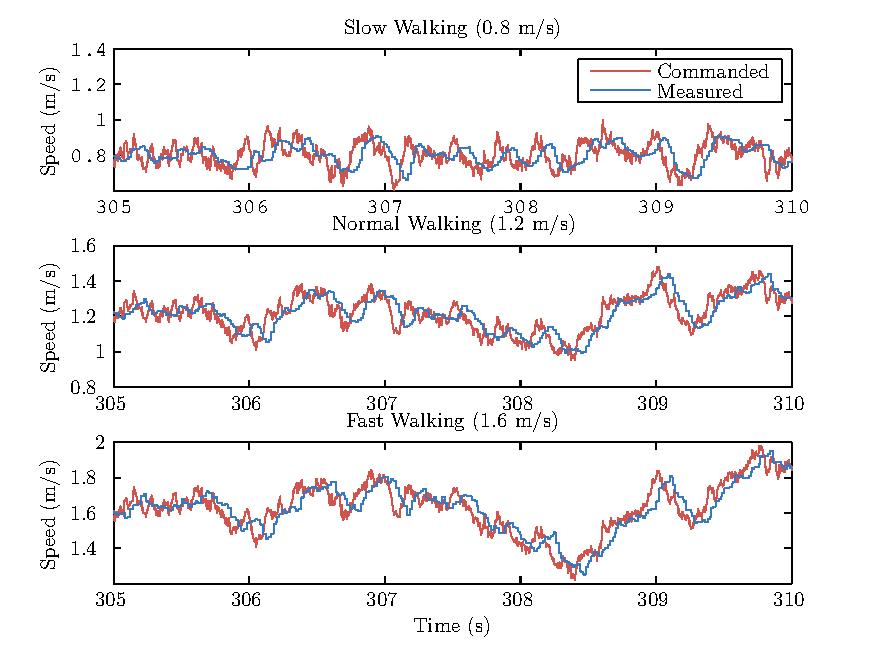
\includegraphics{figures/input_vs_output.pdf}
  \caption{Treadmill belt speed input signals (purple) and recorded output
    speeds (blue) for average belt speeds of
    \SIlist{0.8;1.2;1.6}{\meter\per\second}, respectively.}
  \label{fig:input_output}
\end{figure}

To show the effects of the treadmill dynamics and give an idea of the frequency
content of the actual perturbations, spectral density plots were created 
by averaging a spectrogram over twenty seconds in the Hamming window, shown 
in Figure~\ref{fig:freq_analysis}. For all speeds, the frequency content of the
commanded and measured belt speeds were noticeably similar.  
%
\begin{figure}
  \centering
  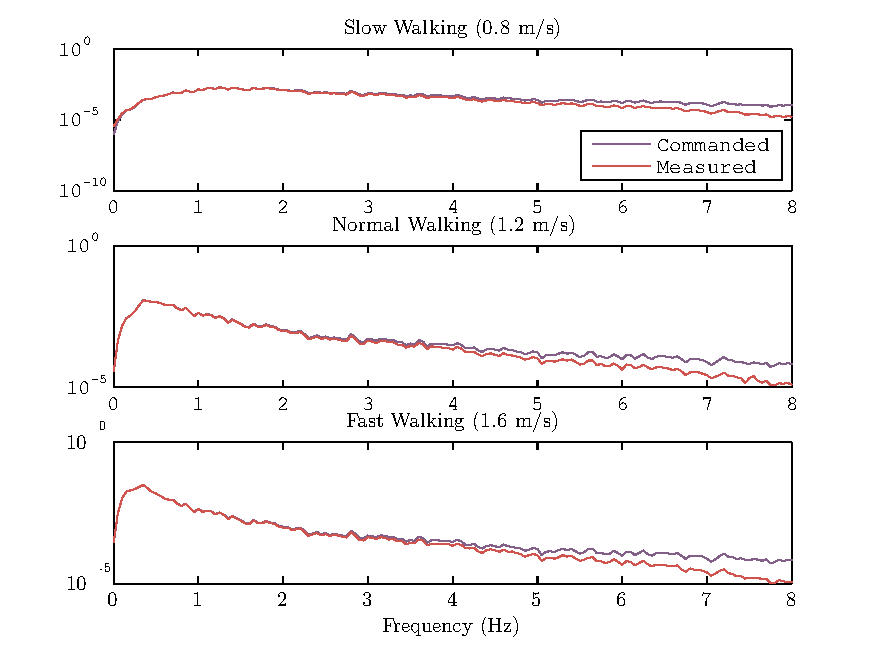
\includegraphics{figures/frequency_analysis.pdf}
  \caption{Frequency spectrum of the treadmill belt velocity input signal
    (purple) and the recorded output velocity (blue) for average belt speeds of
    0.8, 1.2, and 1.6 m/s, respectively}
  \label{fig:freq_analysis}
\end{figure}
\section*{Results}
\subsection*{Raw Data}
%
The raw data consists of a set of ASCII tab delimited text files output from
both the ``mocap'' and ``record'' modules in D-Flow in addition to a manually
generated YAML file that contains all of the necessary meta data for the given
trial. These three files are stored in a hierarchy of directories with one
trial per directory. The directories are named in the following fashion
\verb+T001/+ where \verb+T+ stands for ``trial'' and the following three digits
are provide a unique trial identification number.

\subsubsection*{mocap-xxx.txt}

The output from the D-Flow mocap module is stored in a tab delimited file named
\verb+mocap-xxx.txt+ where \verb+xxx+ represents the trial id number. The file
is tab delimited and contains a number of time series. The numerical values of
the time series are provided in decimal fixed point notation with 6 decimals of
precision, e.g. \verb|123456.123456|, regardless of the units. The first line
of the file holds the header. The header includes time stamp column, frame
number column, marker position columns, force plate force/moment columns, force
plate center of pressure columns, other analog columns, and potentially results
from the real time Human Body Model \cite{Bogert2013} which is included with
D-Flow. The columns are further described below:
%
\begin{description}
  \item[TimeStamp] The monotonically increasing computer clock time when D-Flow
    receives a frame from Cortex. These are recorded at approximately at
    100~\si{\hertz} and given in seconds.
  \item[FrameNumber] Monotonically increasing positive integers that correspond
    to each frame received from Cortex.
  \item[Marker Coordinates] Any column that ends in \verb+.PosX+, \verb+.PosY+,
    or \verb+.PosZ+ are marker coordinates expressed in Cortex's Cartesian
    reference frame. The prefixes match the marker labels given in
    Table~\ref{tab:marker-labels}. These values are in meters.
  \item[Ground Reaction Loads] There are three ground reaction forces and three
    ground reaction moments recorded by each of the two force plates in Newtons
    and Newton-Meters, respectively. The prefix for these columns is either
    \verb+FP1+ or \verb+FP2+ and represents either force plate 1 (left) or 2
    (right). The suffixes are either \verb+.For[XYZ]+, \verb+.Mom[XYZ]+ for the
    forces and moments, respectively. The force plate voltages are sampled at a
    much higher frequency than the cameras, but delivered at the Cortex camera
    sample rate, \~100~\si{\hertz} through the D-Flow mocap module. A
    force/moment calibration matrix stored in Cortex converts the voltages to
    forces and moments before sending it to D-Flow. Cortex also computes
    the center of pressure from the forces, moments, and force plate
    dimensions. These have the same prefixes for the plate number, have the
    suffix \verb+.Cop[XYZ]+, and are given in meters.
  \item[Analog Channels] Several analog signals are recorded under column
    headers \verb+Channel[1-99].Anlg+. These correspond to analog signals
    sampled by Cortex and correspond to the 96 analog channels in the National
    Instruments USB-6255. The first twelve are the voltages from the
    force plate load cells. We also record the acceleration of 4 points on the
    treadmill base in analog channels 61-72 that were in place in case inertial
    compensation for the lateral treadmill movement was required.
\end{description}

\subsubsection*{record-xxx.txt}
%
The record module also outputs a tab delimited ASCII text file with numerical
values at six decimal digits. It includes a \verb+Time+ column which records
the D-Flow system time in seconds. This time corresponds to the time recorded
in the \verb+TimeStamp+ column in mocap module tsv file which is necessary for
time synchronization. There are two additional columns \verb+RightBeltSpeed+
and \verb+LeftBeltSpeed+ which provide the independent belt speeds measured in
meters per second by a factory installed encoder in the treadmill.

Additionally, the record module is capable of recording the time at which
various preprogrammed events occur, as detected or set by D-Flow. It does this
by inserting commented (\verb|#|) lines in between the rows when the event
occurred. The record files have several events that delineate the different
phases of the protocol:
%
\begin{description}
  \item[A: Force Plate Zeroing] Marks the time at the beginning of the trial at
    which there is no load on the force plates and when the force plate
    voltages were zeroed.
  \item[B: Calibration Pose] Marks the time at which the person is in the
    calibration pose.
  \item[C: First Normal Walking] Marks the time when the treadmill begins Phase
    1: constant belt speed.
  \item[D: Longitudinal Perturbation] Marks the time when the treadmill begins
    Phase 2: longitudinal perturbations in the belt speed.
  \item[E: Second Normal Walking] Marks the time when phase 3 starts: constant
    belt speed.
  \item[F: Unloaded End] Marks the time at which there is no load on the force
    plates and the belts are stationary.
\end{description}

\subsubsection*{meta-xxx.yml}

Each trial directory contains a meta data file in the YAML format named in the
following style \verb|meta-xxx.yml| where \verb|xxx| is the three digit trial
identification number. There are three main headings in the file: \verb+study+,
\verb+subject+, and \verb+trial+. An example meta data file is shown in Listing
\ref{lis:example-meta-data}.

The \verb+study+ section contains identifying information for the overall
study, an identification number, name, and description. This is the same for
all meta data files in the study. Details are given below:
%
\begin{description}
  \item[id] An integer specifying a unique identification number of the study.
  \item[name] A string giving the name of the study.
  \item[description] A string with a basic description of the study.
\end{description}

The \verb+subject+ section provides key value pairs of information about the
subject in that trial. Each subject has a unique identification number along
with basic anthropomorphic data. The following details the possible meta data
for the subject:
%
\begin{description}
  \item[age] An integer age in years of the subject at the time of the trial.
  \item[ankle-width-left] A float specifying the width of the subjects left
    ankle.
  \item[ankle-width-right] A float specifying the width of the subjects right
    ankle.
  \item[ankle-width-units] A string giving the units of measurement of the
    ankle widths.
  \item[id] An unique identification integer for the subject.
  \item[gender] A string specifying the gender of the subject.
  \item[height] A float specifying the measured height of the subject (with
    shoes and hat on) at the time of the trial.
  \item[height-units] A string giving the units of the height measurement.
  \item[knee-width-left] A float specifying the width of the subjects left
    knee.
  \item[knee-width-right] A float specifying the width of the subjects right
    knee.
  \item[knee-width-units] A string giving the units of measurement of the
    knee widths.
  \item[mass] A float specifying the self-reported mass of the subject.
  \item[mass-units] A string specifying the units of the mass measurement.
\end{description}

The \verb+trial+ section contains the information about the particular trial.
Each trial has a unique identification number along with a variety of other
information, detailed below:
%
\begin{description}
  \item[analog-channel-map] A mapping of the strings D-Flow assigns to signals
    emitted from the analog channels of the NI USB-6255 to names the user
    desires.
  \item[cortex-version] The version of Cortex used to record the trial.
  \item[datetime] A date formatted string giving the date of the trial in the
    \verb|YYYY-MM-DD| format.
  \item[dflow-version] The version of D-Flow used to record the trial.
  \item[events] A key value map which prescribes names to the alphabetic events
    recorded in the record file.
  \item[files] A key value mapping of files associated with this trial
    where the key is the D-Flow file type and the value is the path to the file
    relative to the meta file. The compensation file corresponds to an unloaded
    trial collected on the same day that could be used for inertial
    compensation purposes, if needed.
  \item[hardware-settings] There are tons of settings for the hardware in both
    D-Flow, Cortex, and the other software in the system. This contains any
    non-default settings.
    \begin{description}
      \item[high-performance] A boolean value indicating whether the D-Flow high
        performance setting was on (True) or off (False).
    \end{description}
  \item[id] An unique three digit integer identifier for the trial. All of the
    file names and directories associated with this trial include this number.
  \item[marker-map] A key value map which maps marker names in the mocap file
    to the user's desired names for the markers.
  \item[marker-set] Indicates the HBM~\cite{Bogert2013} marker set used during
    the trial, either full, lower, or NA.
  \item[nominal-speed] A float representing the nominal desired treadmill speed
    during the trial.
  \item[nominal-speed-units] A string providing the units of the nominal speed.
  \item[notes] Any notes about the trial.
  \item[pitch] A boolean that indicates if the treadmill pitch degree of
    freedom was actuated during the trial.
  \item[stationary-platform] A boolean that indicates whether the treadmill
      sway or pitch motion was actuated during the trial. If this flag is
      false, the measured ground reaction loads must be compensated for the
      inertial affects and be expressed in the motion capture reference frame.
  \item[subject-id] An integer corresponding to the subject in the trial.
  \item[sway] A boolean that indicates if the treadmill lateral degree of
    freedom was actuated during the trial.
\end{description}

\begin{listing}
  \scriptsize
  \begin{minted}[gobble=4]{yaml}
    study:
       id: 1
       name: Gait Control Identification
       description: Perturb the subject during walking and running.
    subject:
       id: 8
       age: 20
       mass: 70.0
       mass-units: kilograms
       height: 1.572
       height-units: meters
       knee-width-left: 107.43
       knee-width-right: 107.41
       knee-width-units: millimeters
       ankle-width-left: 70.52
       ankle-width-right: 67.66
       ankle-width-units: millimeters
       gender: male
    trial:
       id: 58
       subject-id: 8
       datetime: 2014-03-28
       notes: >
           The subject did a somersault during this trial instead of following
           instructions to walk. Will have to use for another study.
       nominal-speed: 0.8
       nominal-speed-units: meters per second
       stationary-platform: True
       pitch: False
       sway: False
       hardware-settings:
           high-performance: True
       dflow-version: 3.16.1
       cortex-version: 3.1.1.1290
       marker-map:
           M1: LHEAD
           M2: THEAD
           M3: RHEAD
           M4: FHEAD
           M5: C7
       analog-channel-map:
           Channel1.Anlg: F1Y1
           Channel2.Anlg: F1Y2
           Channel3.Anlg: F1Y3
           Channel4.Anlg: F1X1
       events:
           A: Force Plate Zeroing
           B: Calibration Pose
           C: First Normal Walking
           D: Longitudinal Perturbation
           E: Second Normal Walking
           F: Unloaded End
       files:
           compensation: ../T057/mocap-057.txt
           mocap: mocap-058.txt
           record: record-058.txt
           meta: meta-058.yml
  \end{minted}
  \caption{A fictitious example of a YAML formatted meta data file. All of the
    possible keys in the data set are shown.}
  \label{lis:example-meta-data}
\end{listing}

\subsection*{Markers}
%
We make use of the full body 47 marker set described in \cite{Bogert2013} and
presented in detail in Table \ref{tab:marker-labels}. As with all camera based
motion capture systems, the markers sometimes go missing in the recording. When
a marker goes missing, if the data was recorded in a D-Flow version less than
3.16.2rc4 [3], D-Flow continues to record the last non-missing value in all
three axes until the marker is visible again. In D-Flow versions greater than
or equal to 3.16.2rc4, the missing markers are indicated in the TSV file as
either \verb|0.000000| or \verb|-0.000000|, which is the same as has been in
the HBM columns in all versions of D-Flow. The D-Flow version must be provided
in the meta data yml file for each trial to be able to distinguish this detail.
%
\begin{table*}
  \cprotect\caption{Descriptions of the 47 markers used in this study. The
    ``Set'' column indicates whether the marker exists in the lower and/or full
    body marker set. The label column matches the column headers in the
    \verb|mocap-xxx.txt| files and/or the marker map in the \verb|meta-xxx.yml|
    file.}
  \centering
  \footnotesize
  \begin{tabular}{lrlll}
    \toprule
    Set & \# & Label & Name & Description \\
    \midrule
    F   & 1  & LHEAD & Left head                             & Just above the ear, in the middle. \\
    F   & 2  & THEAD & Top head                              & On top of the head, in line with the LHEAD and RHEAD. \\
    F   & 3  & RHEAD & Right head                            & Just above the ear, in the middle. \\
    F   & 4  & FHEAD & Forehead                              & Between line LHEAD/RHEAD and THEAD a bit right from center. \\
    L/F & 5  & C7    & C7                                    & On the 7th cervical vertebrae. \\
    L/F & 6  & T10   & T10                                   & On the 10th thoracic vertbrae. \\
    L/F & 7  & SACR  & Sacrum bone                           & On the sacral bone. \\
    L/F & 8  & NAVE  & Navel                                 & On the navel. \\
    L/F & 9  & XYPH  & Xiphoid process                       & Xiphoid process of the sternum. \\
    F   & 10 & STRN  & Sternum                               & On the jugular notch of the sternum. \\
    F   & 11 & BBAC  & Scapula                               & On the inferior angle fo the right scapular. \\
    F   & 12 & LSHO  & Left shoulder                         & Left acromion. \\
    F   & 13 & LDELT & Left deltoid muscle                   & Apex of the deltoid muscle. \\
    F   & 14 & LLEE  & Left lateral elbow                    & Left lateral epicondyle of the elbow. Upper one in the T-Pose. \\
    F   & 15 & LMEE  & Left medial elbow                     & Left medial epicondyle of the elbow. Lower on in the T-Pose. \\
    F   & 16 & LFRM  & Left forearm                          & On 2/3 on the line between the LLEE and LMW. \\
    F   & 17 & LMW   & Left medial wrist                     & On styloid process radius, thumb side. \\
    F   & 18 & LLW   & Left lateral wrist                    & On styloid process ulna, pinky side. \\
    F   & 19 & LFIN  & Left fingers                          & Center of the hand. Caput metatarsal 3. \\
    F   & 20 & RSHO  & Right shoulder                        & Right acromion. \\
    F   & 21 & RDELT & Right deltoid muscle                  & Apex of deltoid muscle. \\
    F   & 22 & RLEE  & Right lateral elbow                   & Right lateral epicondyle of the elbow. Lower one in the T-pose. \\
    F   & 23 & RMEE  & Right medial elbow                    & Right medial epicondyle of the elbow. Lower one in the T-pose. \\
    F   & 24 & RFRM  & Right forearm                         & On 1/3 on the line between the RLEE and RMW. \\
    F   & 25 & RMW   & Right medial wrist                    & On styloid process radius, thumb side. \\
    F   & 26 & RLW   & Right lateral wrist                   & On styloid process ulna, pinky side. \\
    F   & 27 & RFIN  & Right fingers                         & Center of the hand. Caput metatarsal 3. \\
    L/F & 28 & LASIS & Pelvic bone left front                & Left anterior superior iliac spine. \\
    L/F & 29 & RASIS & Pelvic bone right front               & Right anterior superior iliac spine. \\
    L/F & 30 & LPSIS & Pelvic bone left back                 & Left posterior superio iliac spine. \\
    L/F & 31 & RPSIS & Pelvic bone right back                & Right posterior superior iliac spine. \\
    L/F & 32 & LGTRO & Left greater trochanter of the femur  & On the cetner of the left greater trochanter. \\
    L/F & 33 & FLTHI & Left thigh                            & On 1/3 on the line between the LFTRO and LLEK. \\
    L/F & 34 & LLEK  & Left lateral epicondyle of the knee   & On the lateral side of the joint axis. \\
    L/F & 35 & LATI  & Left anterior of the tibia            & On 2/3 on the line between the LLEK and LLM. \\
    L/F & 36 & LLM   & Left lateral malleoulus of the ankle  & The center of the heel at the same height as the toe. \\
    L/F & 37 & LHEE  & Left heel                             & Center of the heel at the same height as the toe. \\
    L/F & 38 & LTOE  & Left toe                              & Tip of big toe. \\
    L/F & 39 & LMT5  & Left 5th metatarsal                   & Caput of the 5th metatarsal bone, on joint line midfoot/toes. \\
    L/F & 40 & RGTRO & Right greater trochanter of the femur & On the cetner of the right greater trochanter. \\
    L/F & 41 & FRTHI & Right thigh                           & On 2/3 on the line between the RFTRO and RLEK. \\
    L/F & 42 & RLEK  & Right lateral epicondyle of the knee  & On the lateral side of the joint axis. \\
    L/F & 43 & RATI  & Right anterior of the tibia           & On 1/3 on the line between the RLEK and RLM. \\
    L/F & 44 & RLM   & Right lateral malleoulus of the ankle & The center of the heel at the same height as the toe. \\
    L/F & 45 & RHEE  & Right heel                            & Center of the heel at the same height as the toe. \\
    L/F & 46 & RTOE  & Right toe                             & Tip of big toe. \\
    L/F & 47 & RMT5  & Right 5th metatarsal                  & Caput of the 5th metatarsal bone, on joint line midfoot/toes. \\
    \bottomrule
  \end{tabular}
  \label{tab:marker-labels}
\end{table*}

\subsection*{Processed Data}
%
We developed a toolkit for data processing, GaitAnalysisToolKit v0.1.2,
\cite{Moore2014a}, for common gait computations and provide an example
processed trial to present the nature of the data. The tool was developed in
Python, is dependent on the SciPy Stack and Octave, and provides two main
classes: one to do basic gait data cleaning from D-Flow's output files,
\verb|DFlowData|, and a second to compute common gait variables of interest,
\verb|GaitData|.

The \verb|DFlowData| class collects and stores all the raw data presented in
the previous section and applies several ``cleaning'' operations to transform
the data into a usable form. The cleaning process follows these steps:
%
\begin{enumerate}
  \item Load the meta data file into a Python dictionary.
  \item Load the D-Flow mocap module TSV file into Pandas \verb|DataFrame|.
  \item Relabel the column headers to more meaningful names if this is
    specified in the meta data.
  \item Optionally identify the missing values in the mocap marker data and
    replace them with \verb|numpy.nan|.
  \item Optionally interpolate the missing marker values and replaces them
    with interpolated estimates using a variety of interpolation methods.
  \item Load the D-Flow record module TSV file into a Pandas \verb|DataFrame|.
  \item Extract the events and create a dictionary mapping the event names in
    the meta data to the events detected in the record module file.
  \item Interially compensate the ground reaction loads based on whether the
    meta data indicates there was treadmill motion.
  \item Merge the data from the mocap module and record module into one data
    frame at the maximum common constant sample rate.
\end{enumerate}

Once the data is cleaned there are two methods that allow you to extract the
cleaned data: either extract sections of the data bounded by the events
recorded in the \verb|record-xxx.txt| file or save the cleaned data to disk.
These operations are available as a command line application and as an
application programming interface (API) in Python. An example of the
\verb|DFlowData| API in use is provided in Listing~\ref{lis:dflowdata}.
%
\begin{listing}
  \begin{minted}[gobble=4]{python}
    >>> from gaitanalysis.motek import DFlowData
    >>> data = DFlowData('mocap-020.txt', 'record-020.txt',
    ...                  'meta-020.yml')
    >>> mass = data.meta['subject']['mass']
    >>> data.clean_data()
    >>> event_df =data.extract_processed_data(
    ...     event='Longitudinal Perturbation')
  \end{minted}
  \cprotect\caption{Python interpreter session showing how one could load a
    trial into memory, extract the subject's mass from the meta data, run the
    data cleaning process, and finally extract a Pandas \verb|DataFrame|
    containing all of the time histories for a specific event in the trial.}
  \label{lis:dflowdata}
\end{listing}

The \verb|GaitData| class is then used to compute things such as gait events
(toe off and heel strike times), basic 2D kinematics and inverse dynamics, and
to store the data into a Pandas \verb|Panel| with each gait cycle on the item
axis at a specified sample rate. This object can also be serialized to disk in
HDF5 format. An example of using the Python API is shown in
Listing~\ref{lis:gaitdata}.
%
\begin{listing}
  \begin{minted}[gobble=4]{python}
    >>> from gaitanalysis.gait import GaitData
    >>> gdata = GaitData(event_df)
    >>> gdata.inverse_dynamics_2d(left_markers, right_markers,
    ...                           left_loads, right_loads, mass, 6.0)
    >>> gdata.grf_landmarks('Right Fy', 'Left Fy', threshhold=20.0)
    >>> gdata.split_at('right')
    >>> gdata.plot_gait_cycles('Left Hip Joint Torque', mean=True)
    >>> gdata.save('gait-data.h5')
  \end{minted}
  \cprotect\caption{Python interpreter session showing how one could use the
    \verb|GaitData| class to load in the result of \verb|DFlowData| and compute
    the inverse dynamics (joint angles and torques), identify the gait events
    (e.g. heel strikes), split the data with respect to the gait events into a
    Pandas \verb|Panel|, plot the mean and standard deviation of one time
    history with respect to the gait cycles, and save the data to disk.}
  \label{lis:gaitdata}
\end{listing}

A similar work flow was used to produce Figure~\ref{fig:angle-torque-comparison}
which compares the mean and standard deviation of sagittal plane joint angles
and torques from the perturbed gait cycles and the unperturbed gait cycles
computed from trial 20. This gives an idea of the more highly variable dynamics
required to walk while being longitudinally perturbed.
%
\begin{figure}
  \centering
  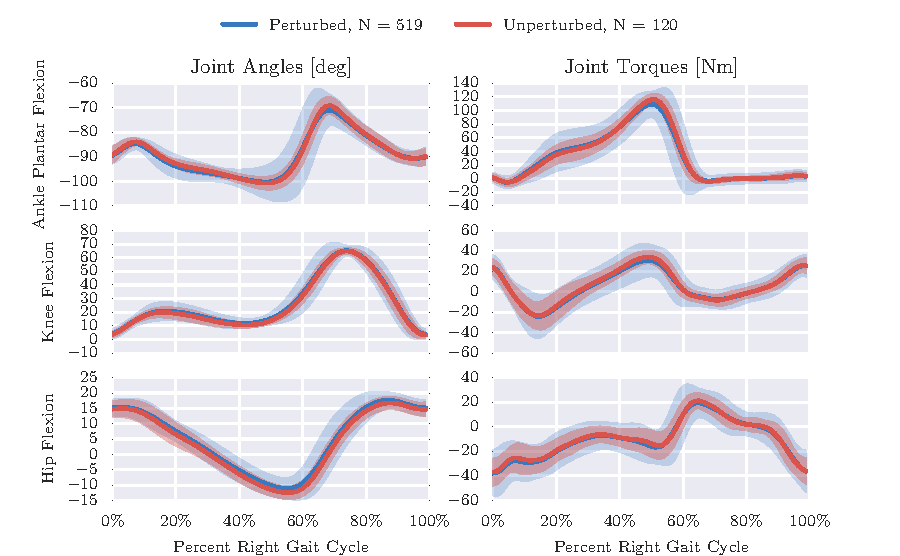
\includegraphics{figures/unperturbed-perturbed-comparison.pdf}
  \cprotect\caption{Mean (right: solid, left: dashed) and $3\sigma$ (shaded)
    joint angles and torques from both unperturbed (purple) and perturbed
    (blue) gait cycles from trial 20. Produced by
    \verb|src/unperturbed_perturbed_comparison.py|.}
  \label{fig:angle-torque-comparison}
\end{figure}

For more insight into the difference in the unperturbed and perturbed data,
Figure~\ref{fig:gait-cycle-stats-comparison} compares the distribution of a few
gait cycle statistics. One can see that the perturbed strides have a much
larger variation in frequency and length.
%
\begin{figure}
  \centering
  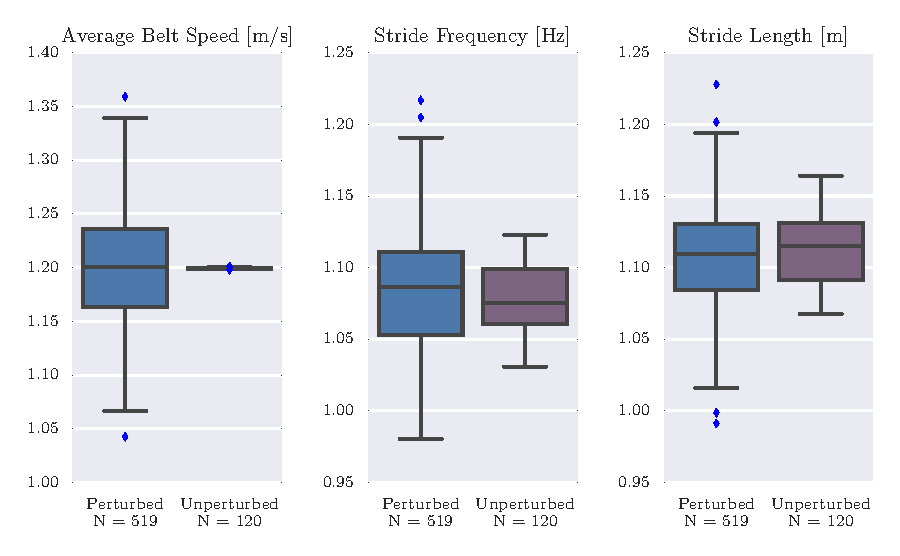
\includegraphics{figures/unperturbed-perturbed-boxplot-comparison.pdf}
  \cprotect\caption{Box plots of the average belt speed, stride frequency, and
    stride length which compare unperturbed (purple) and perturbed (blue) gait
    cycles. The median is given with the box bounding the first and third
    quartiles and the whiskers bound the range of the data. Produced by
    \verb|src/unperturbed_perturbed_comparison.py|.}
  \label{fig:gait-cycle-stats-comparison}
\end{figure}

\subsection*{Data Limitations}
%
The data is provided in good faith with great attention to detail but as with
all data there are anomalies that may affect the use and interpretation of
results emanating from the data. The following list gives various notes and
warnings about the data that should be taken into account when making use of
it.
%
\begin{itemize}
  \item Be sure to read the notes in each meta data file for details about
    possible anomalies in that particular trial. Things such as marker dropout,
    ghost markers, and marker movement are the more prominent notes. Details
    about variations in the equipment on the day of the trial are also
    mentioned.
  \item The subject identification number 0 stands for "no subject" and was
    used whenever data was collected from the system with no subject on the
    treadmill, for example during the trials that were intended to be used for
    inertial compensation purposes. These trials play through the exact
    protocol as those with a human subject and the matching trials are
    indicated in the meta data. Matching unloaded trials were recorded on the
    same day as the loaded trials and is noted in the
    \verb|trial:files:compensation| section of the meta data file.
  \item Trials 1 and 2 were not recorded as part of this study. Those trial
    identification numbers were reserved for early data exploration from data
    collected in other studies.
  \item Trials 37, 38, and 39 do not exist. The numbers were accidentally
    skipped.
  \item Trials 9, 10, and 11 used a slightly different event definition where the
    calibration poses were not explicitly tagged by an event, yet the protocol
    was the identical to the following trials. The calibration pose will have
    to be determined manually.
  \item  Trials 6-15 have force measurements are affected by the treadmill
    vibration mode mentioned in the equipment section and the forces should be
    not be used. We include the trials because both the kinematic data is valid
    and trials 6-8 include lateral perturbations in addition to the
    longitudinal.
  \item During trials 9-15 we used wooden blocks to fix the treadmill to the
    concrete floor to eliminate the treadmill's low vibration mode
    (approximately 5\si{\hertz}). But these blocks seem to have corrupted the
    force plate measurements by imposing frictional stresses on the system. The
    force plate measurements should not be used from these trials, but the
    marker data is fine.
  \item Trials 6-8 use an early experimental protocol which divided the
    perturbation sections into three sections: longitudinal perturbations,
    lateral perturbations, and a combination of each. We then learned the
    treadmill had a low vibrational mode which significantly affects the force
    plate measurements, requiring us to eliminate the lateral perturbation
    motions. The force measurements during these trials are corrupted by this
    vibrational mode and should be used with caution or not at all.
  \item We did not record unloaded compensation trials for trials 9-15.
    Regardless, they would likely be useless due to the corruption from the
    wooden blocks.
  \item Trials 6-8 use a only the lower body marker set. The remaining trials
    are full body.
  \item The ankle joint torques computed from subject 9's data in trials 25-27
    are abnormal and should be used with caution or not at all. We were not
    able to locate the source of the error, but it is likely related to the
    force calibration.
\end{itemize}

\section*{Conclusion}
%
We have presented a rich and elaborate data set of motion and ground reaction
loads from human subjects during both normal walking and when recovering from
longitudinal perturbations. The raw data is provided for reuse with complete
meta data. In addition to the data, we provide software that can process the
data for both cleaning purposes and to produce typical sagittal plane gait
variables of interest. Among other uses, we believe the dataset is ideally
suited for control identification purposes. Many researchers are working on
mathematical models for control in gait and this dataset provides both a way to
validate these models and a source for generating them.

\section*{Data Availability}
The data set, \cite{Moore2014}, is available via the Zenodo data repository.
Two approximately 1.2GB gzipped tar balls contain the data and a \verb|README|
file with a short description of the contents. The data is released under the
Creative Commons CC0 license (http://creativecommons.org/about/cc0) following
best practices for sharing scientific data.

\section*{Software Availability}
The tables and figures in the paper can be reproduced from the source
repository shared on Github: https://github.com/csu-hmc/perturbed-data-paper.
Along with the source code in the repository, the computations depend on
version 0.1.2 of the GaitAnalysisToolKit, \cite{Moore2014a}, which can be
downloaded from Zenodo or the Python Package Index (http://pypi.python.org).

\section*{Author contributions}
A.v.d.B. conceived of the experiments and protocol. J.K.M and S.K.H refined the
protocol, ran the experiments, collected the data, developed the software, and
analyzed the data. J.K.M was the primary author of the paper with significant
contributions from S.K.H and A.v.d.B. All authors were involved in the revision
of the draft manuscript and have agreed to the final content.

\section*{Competing interests}
The authors have no financial, personal, or professional competing interests
that could be construed to unduly influence the content of this article.

\section*{Grant Information}
The work was partially funded by the State of Ohio Third Frontier Commission
through the Wright Center for Sensor Systems Engineering (WCSSE) and by the
National Science Foundation under Grant No. 1344954.

\section*{Acknowledgments}
%
We thank Roman Boychuk and Obinna Nwanna for assistance with the experiments.
We also thank Sabrina Abram, Brad Humphreys, and Anne Koelewijn for reviewing
the preprint and being our guinea pigs on the software/data instructions. Dan
Simon also gave valuable feedback on the preprint.

\bibliography{gait-data}

\end{document}
